% ----------------------------------------------------------
\chapter{Introdução}
% ----------------------------------------------------------

%As orientações aqui apresentadas são baseadas em um conjunto de normas elaboradas pela \gls{ABNT}. Além das normas técnicas, a Biblioteca também elaborou uma série de tutoriais, guias, \textit{templates} os quais estão disponíveis em seu site, no endereço \url{http://portal.bu.ufsc.br/normalizacao/}.

%Paralelamente ao uso deste \textit{template} recomenda-se que seja utilizado o \textbf{Tutorial de Trabalhos Acadêmicos} (disponível neste link \url{https://repositorio.ufsc.br/handle/123456789/180829}) e/ou que o discente \textbf{participe das capacitações oferecidas da Biblioteca Universitária da UFSC}.

%Este \textit{template} está configurado apenas para a impressão utilizando o anverso das folhas, caso você queira imprimir usando a frente e o verso, acrescente a opção \textit{openright} e mude de \textit{oneside} para \textit{twoside} nas configurações da classe \textit{abntex2} no início do arquivo principal \textit{main.tex} \cite{abntex2classe}.

%Os trabalhos de conclusão de curso (TCC) de graduação e de especialização não são entregues em formato impresso na Biblioteca Universitária. Porém, sua versão PDF pode ser disponibilizada no Repositório Institucional, consulte seu curso sobre os procedimentos adotados para a entrega. 

%\nocite{NBR6023:2002}
%\nocite{NBR6027:2012}
%\nocite{NBR6028:2003}
%\nocite{NBR10520:2002}

% ----------------------------------------------------------
%\section{Recomendações de uso}
% ----------------------------------------------------------

%Este \emph{template} foi elaborado para se compilado em \LaTeX utilizando \abnTeX.  Todas as configurações de diferenciação gráfica nas divisões de seção e subseção seguem a  norma NBR 6027/2012 automaticamente. 

%Uma nota de rodapé, já tem seu estilo automático com o comando \texttt{$\backslash$footnote}\footnote{As notas de rodapé possuem fonte tamanho 10. O alinhamento das linhas da nota de rodapé deve ser abaixo da primeira letra da primeira palavra da nota de modo dar destaque ao expoente.}.

O consumo e compartilhamento de conteúdos em vídeo vem aumentando consideravelmente nos últimos anos.
Atualmente se estima que vídeos sejam responsáveis por 71\% de todo o tráfego de dados móveis, e a previsão é que esse valor aumente para 80\% até 2028 \cite{mobile}.
Ao se considerar um panorama mais amplo, há dados apontando que conteúdo em vídeo representou quase 66\% do volume total de tráfego na Internet no primeiro semestre de 2022 \cite{traffic}, havendo aumento de 24\% em relação ao mesmo período de 2021.

Tendo em vista esse cenário, fica evidente a importância da codificação de vídeos, a qual busca formas de armazenar, transmitir e reproduzir esse tipo de dado de forma otimizada.
Nesse contexto, a abordagem mais consolidada é a codificação híbrida, a qual vem sendo parte essencial do estado da arte da área nas últimas décadas.
Os padrões de codificação híbridos valem-se de diferentes técnicas para examinar quadros e regiões dentro dos quadros a procura de informações redundantes para o sistema visual humano. Com isso, eles exploram a taxa de compressão atingida para minimizar tanto quanto possível o armazenamento, mantendo ao máximo a qualidade.
Contudo, o aumento da demanda e da concorrência observado recentemente tem levado ao desenvolvimento de algoritmos cada vez mais complexos, impactando no custo computacional e no tempo de execução.
Dessa maneira, a cada geração, a eficiência de codificação vem duplicando, ao custo de um aumento na complexidade de cerca de 10X.
Por consequência, técnicas alternativas têm sido propostas para tentar melhorar a eficiência de codificação, e uma delas é o \ac{DIVC} \cite{ours}.
Esse modelo de codificação consiste em combinar o uso de um dos padrões híbridos com a realização de \ac{VFI}.

\ac{VFI} é uma técnica para gerar ao menos um quadro intermediário ($Q_t$), tomando como referência pelo menos um quadro anterior ($Q_0$) e um posterior ($Q_1$), como mostra a Figura \ref{fig:vfi}.
Nesse caso, \textit{t} representa a posição temporal do quadro interpolado em relação aos quadros de referência, com $0<t<1$.
Os quadros podem ser produzidos com diferentes propósitos, e as implementações mais recentes são baseadas na utilização de \acp{NN}.
Uma das abordagens mais empregadas pode ser classificada como \textit{flow-based}, e consiste em computar o \textit{optical flow}, o qual é usado para relizar \textit{warping} sobre os quadros de referência.
Um exemplo desse tipo de arquitetura foi proposto por \textcite{niklaus2020softmax}.

\begin{figure}[htb]
    \centering
    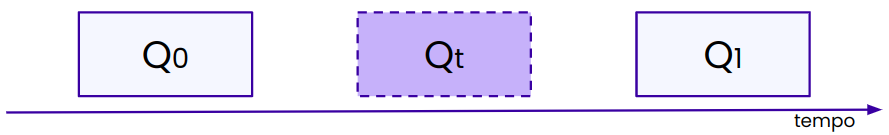
\includegraphics[width=0.8\columnwidth,keepaspectratio]{images/vfi1.png}
    \caption{Interpolação de Quadros de Vídeo - \textit{Video Frame Interpolation} (VFI). Fonte: Elaborado pela autora.}
    \label{fig:vfi}
\end{figure}

Dessa forma, a abordagem \ac{DIVC} propõe retirar os quadros de índice par do vídeo (riscados em vermelho na Figura \ref{fig:divc}) e codificar os quadros de índice ímpar com o método tradicional. Após a etapa de decodificação, \ac{VFI} é usado para regerar os quadros pares a partir dos quadros ímpares reconstruídos. Entretanto, um problema relacionado à aplicação dessa técnica que se observa a partir dos testes realizados é que os resultados variam muito em função do conteúdo do vídeo \cite{ours}.

\begin{figure}[htb]
    \centering
    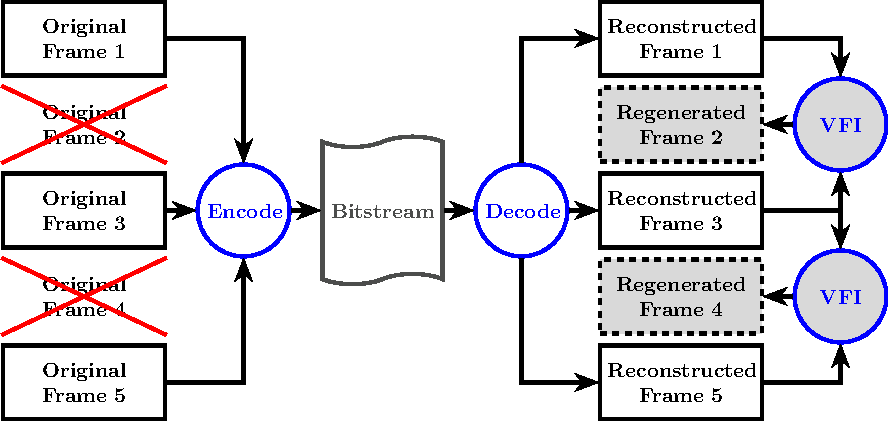
\includegraphics[width=0.8\columnwidth,keepaspectratio]{images/hybrid_vfi.pdf}
    \caption{\textit{Decoupled Interpolated Video Coding} (DIVC). Fonte: \textcite{ours}.}
    \label{fig:divc}
\end{figure}

Um tipo de ferramenta que pode ser útil para identificar características e conteúdos presentes em imagens e vídeos são os descritores \cite{Kumar2014ASO}. Eles podem ser utilizados para inúmeras aplicações, como reconhecimento de padrões, rastreamento e identificação de objetos. Um exemplo de descritor conhecido na literatura é o \ac{ORB} \cite{orb}, que foi desenvolvido tendo como foco diversas aplicações, como detecção de objetos e \textit{patch-tracking}. Outro exemplo é o \ac{FREAK} \cite{freak}, o qual foi projetado tendo inspiração no \ac{SVH}.

Assim, especula-se que seja possível melhorar a eficiência de codificação do \ac{DIVC} a partir da remoção de quadros de maneira adaptativa. Essa remoção poderia ser feita considerando características do conteúdo, as quais seriam obtidas com o auxílio de descritores de imagem e/ou vídeo.

%Inicialmente nesse relatório discute-se sobre o referencial teórico básico dos algoritmos de aprendizado de máquina que foram utilizados, juntamente com a explicação dos cálculos matemáticos que são feitos nas predições dos modelos. Depois, explicam-se os métodos utilizados para se extrair os dados que treinaram os algoritmos, assim como as técnicas aplicadas em suas modelagens para evitar problemas de \textit{overfit} e melhorar a performance dos modelos tomando como base a função de custo escolhida. Logo em seguida os resultados dos treinamentos são discutidos por meio tanto da análise dos erros da predições quanto pela representação gráfica mais intuitiva desses erros. Por fim, sintetiza-se todo o processo realizado e os resultados obtidos em uma conclusão que indica qual foi o melhor algoritmo e o pior algoritmo para o objetivo posto nesse trabalho. 


% ----------------------------------------------------------
\section{Objetivos}
% ----------------------------------------------------------

%Nas seções abaixo estão descritos o objetivo geral e os objetivos específicos deste TCC.

% ----------------------------------------------------------
% São objetivos gerais e especificos deste trabalho: 


% \subsection*{Objetivo Geral}
% % ----------------------------------------------------------

%Neste panorama, este trabalho de conclusão de curso tem dois objetivos principais. Em primeiro momento, propõe-se a utilizar técnicas de \gls{AxC} para desenvolver e avaliar um conjunto de comparadores aproximados seguindo figuras de mérito estabelecidos na literatura. Posteriormente, busca fornecer um fluxo de projeto para determinação das técnicas de aproximação mais apropriadas para comparadores no contexto de aplicações de classificação com \gls{DT}s, de modo a otimizar a relação entre dissipação de potência e acurácia.

O objetivo geral deste trabalho é melhorar a eficiência de codificação do modelo \ac{DIVC} através da remoção de quadros de vídeos de forma adaptativa.
Para essa finalidade, pretende-se utilizar diferentes descritores de imagem e/ou vídeo para extrair características das sequências as quais tenham potencial influência na qualidade dos resultados obtidos com a aplicação do \ac{DIVC}.


% ----------------------------------------------------------
\subsection*{Objetivos Específicos}
% ----------------------------------------------------------

\begin{itemize}
    \item Determinar quais descritores de imagem/vídeo apresentam melhor correlação com a eficiência de codificação na utilização do método \ac{DIVC};
    \item Melhorar a eficiência de codificação do modelo \ac{DIVC} através da remoção adaptativa de quadros, a partir da avaliação dos mesmos por meio dos descritores escolhidos.
\end{itemize}
% ----------------------------------------------------------	
